\section*{Lectura 5: Homotop\'ia.}

\begin{definition}
    Sean $X$ y  $Y$ espacios topologicos, y sean  $f_0:X \xrightarrow{} Y$ y
    $f_1:X \xrightarrow{} Y$ mapas continuas. Decimos que $f_0$ es
    \textbf{homot\'opico} a $f_1$ s\'i existe una mapa continua $F:X \times I
    \xrightarrow{} Y$ tal que $F(x,0)=f_0(x)$ y $F(x,1)=f_1(x)$ para todo $X \in
    X$. Decimos que  $f_0$ y $f_1$ son \textbf{homot\'opicos} y escribimos $f_0
    \simeq f_1$.
\end{definition}

\begin{figure}[h]
    \centering
    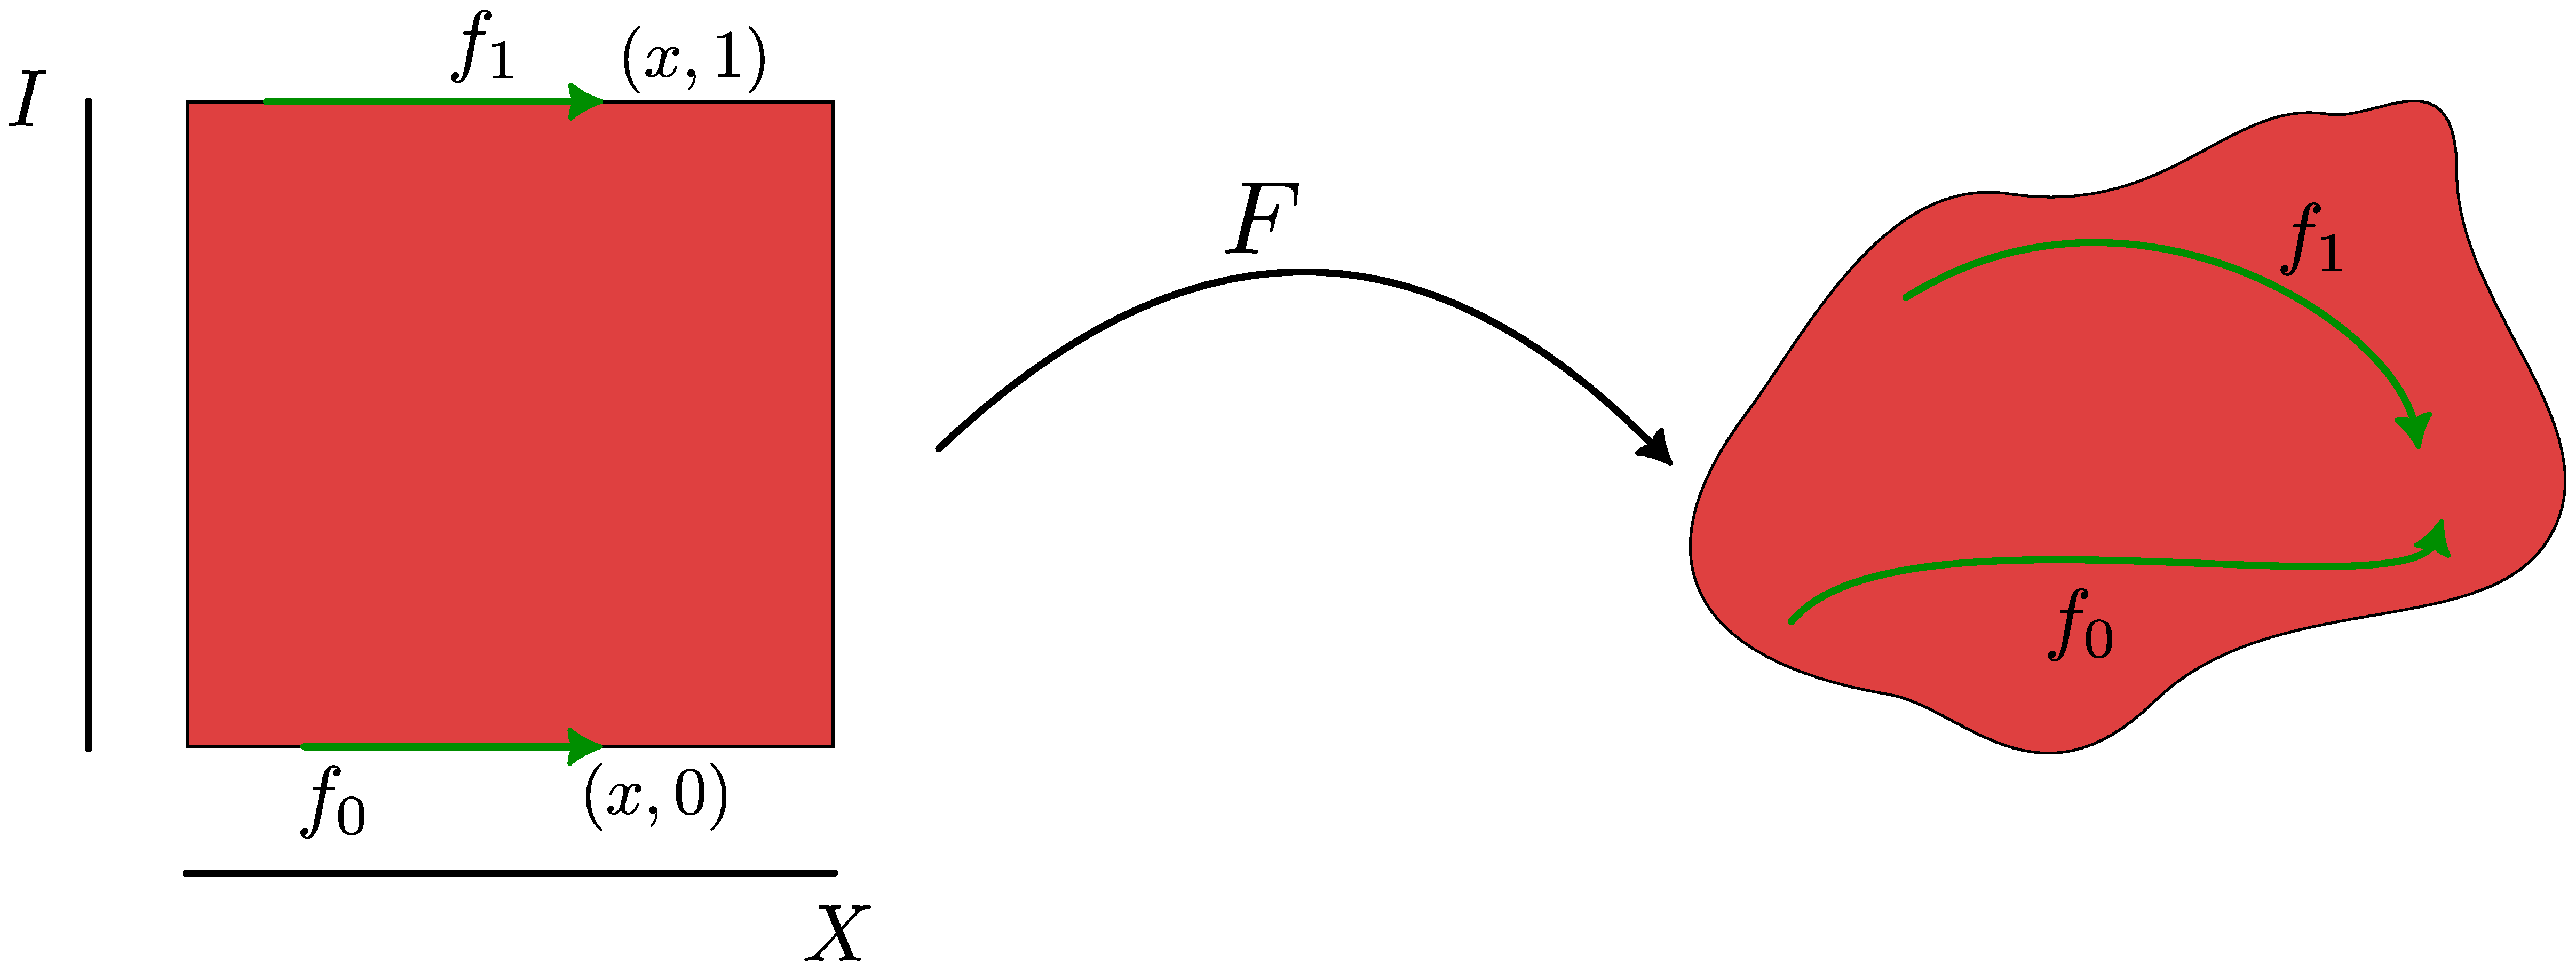
\includegraphics[scale=0.2]{Figures/homotopia.eps}
    \caption{Dos mapas continuas $f_0$ y $f_1$ homot\'opicos.}
    \label{fig_13}
\end{figure}

\begin{theorem}[Primer Teorema de Empaste]\label{thm_5.6}
    Sean $X$ y  $Y$ espacios topologicos y  $f:X \xrightarrow{} Y$ una mapa.
    Entonces:
    \begin{enumerate}
        \item[(1)] S\'i $\{U_\alpha\}$ es una colecci\'on de conjuntos abiertos
            de $X$ con  $X=\bigcup{U_\alpha}$, tal que $f|_{U_\alpha}$ es
            continua, entonces $f$ es continua.

        \item[(2)] S\'i $\{U_\alpha\}$ es una colecci\'on de conjuntos cerrados
            de $X$ con  $X=\bigcup{U_\alpha}$, tal que $f|_{U_\alpha}$ es
            continua, entonces $f$ es continua.
    \end{enumerate}
\end{theorem}

\begin{lemma}[Segundo Teorema de Empaste]\label{lemma_5.7}
    Sea $X$ un espacio topologico que es una union finita de conjuntos
    cerrados en $X$, $X=\bigcup_{i=1}^n{X_i}$. S\'i $Y$ es un espacio y
    $\{f_i\}_{i=1}^n$ una coleccion de mapas $f_i:X_i \xrightarrow{} Y$
    continuas que coincidan en la intersecci\'on, entonces existe una mapa
    continua $f:X \xrightarrow{} Y$ tal que $f|_{X_i}=f_i$.
\end{lemma}
\begin{proof}
    Considere la mapa $f(x)=f_i(x)$ para todo $x \in X_i$. Entonces $f$ coincida
    en la intersecci\'on con todo $f_i$, as\'i que es bien definida, y es claro
    que $f|_{X_i}=f_i$.

    Ahora sea $C$ un conjunto cerrado en  $Y$. Entonces  $\inv{f}(C)=X \cap
    \inv{f}(C)=\bigcup_{i=1}^n{X_i} \cap \inv{f}(C)=\bigcup_{i=1}^n{(X_i \cap
    f(C))}=\bigcup{(X_i \cap \inv{f_i}(C))}$. Ahora, $X_i$ y $\inv{f_i}$ est\'an
    cerrados as\'i que  $X_i \cap \inv{f_i}(X)$ es cerrado. Entonces el union
    finita de ellos para todo $i$ es cerrado, as\'i que $\inv{f}(C)$ es cerrado
    en $X$, lo cual hace  $f$ continua.
\end{proof}

\begin{lemma}[Tercer Teorema de Empaste]\label{lemma_5.8}
    Sea $X$ un espacio topologico que es una union arbitraria de conjuntos
    abiertos en $X$, $X=\bigcup{X_\alpha}$. S\'i $Y$ es un espacio y
    $\{f_\alpha\}$ una coleccion de mapas $f_\alpha:X_\alpha \xrightarrow{} Y$
    continuas que coincidan en la intersecci\'on, entonces existe una mapa
    continua $f:X \xrightarrow{} Y$ tal que $f|_{X_\alpha}=f_\alpha$.
\end{lemma}

\begin{lemma}\label{lemma_5.9}
    La homotop\'ia es una relaci\'on de equivalencia sobre mapas continuas.
\end{lemma}
\begin{proof}
    Sea $X$ y $Y$ espacios topologicos. Sea $f:X \xrightarrow{} Y$ una
    mapa continua y define $F:X \times I \xrightarrow{} Y$ con $F(x,t)=f(x)$
    para todo $(x,t) \in X \times I$. Nota que para alg\'un mapa continua $h:X
    \times I \xrightarrow{} X \times I$, que $F=\pi_1 \circ h$ donde $\pi_1$ es
    la proyecci\'on de la primer parte.$F$ es continua porque es la
    composici\'on de mapas continuas. Entonces vemos que $(x,t)
    \xrightarrow{h} (f(x),t) \xrightarrow{\pi_1} \xrightarrow{} f(x)$. Entonces
    podemos ver que $F(x,0)=F(x,1)=f(x)$, as\'i que $f \simeq f$.

    Ahora considere  $f:X \xrightarrow{} Y$, y $g:Y \xrightarrow{} Z$ continuas
    tal que $f \simeq g$. Sea  $F:X \times I \xrightarrow{} Y$ la homotop\'ia de
    esos dos mapas. Entonces $F(x,0)=f(x)$ y $F(x,1)=g(x)$. Defina la mapa $G:X
    \times I \xrightarrow{} Y$ dado por $G(x,t)=F(x,1-t)$. Como $G$ solo
    transforma coordinadas, $G$ es continua. Entonces vemos que
    $G(x,0)=F(x,1)=g(x)$ y $G(x,1)=F(x,0)=f(x)$; as\'i que $g \simeq f$.

    Por ultimo, sea  $f:X \xrightarrow{} Y$, $g:X \xrightarrow{} Y$ y $h:X
    \xrightarrow{} Y$ mapas continuas tales que $f \simeq g$ y $g \simeq h$.
    Entonces existe homotopias  $F:X \times I \xrightarrow{} Y$ y $G:X \times I
    \xrightarrow{} Y$ con $F(x,0)=f(x)$, $F(x,1)=g(x)$ y $G(x,0)=g(x)$,
    $G(x,1)=h(x)$. Considere la mapa $H:X \times I \xrightarrow{} Y$ dado por:
    \begin{equation*}
        H(x,t)=\begin{cases}
                F(x,2t), \text{ s\'i} 0 \leq t \leq \frac{1}{2} \\
                G(x,2t-1), \text{ s\'i } \frac{1}{2} \leq t \leq 1  \\
               \end{cases}
    \end{equation*}
    Vemos que los dominios de $F$ y $H$ coninciden, y que son continuas. As\'i
    que por la teorema del empaste, $H$ es continua. Entonces vemos que
    $H(x,0)=F(x,0)=f(x)$ y que $H(x,1)=G(x,1)=h(X)$ lo que hace $f \simeq h$.
\end{proof}

\begin{figure}[h]
    \centering
    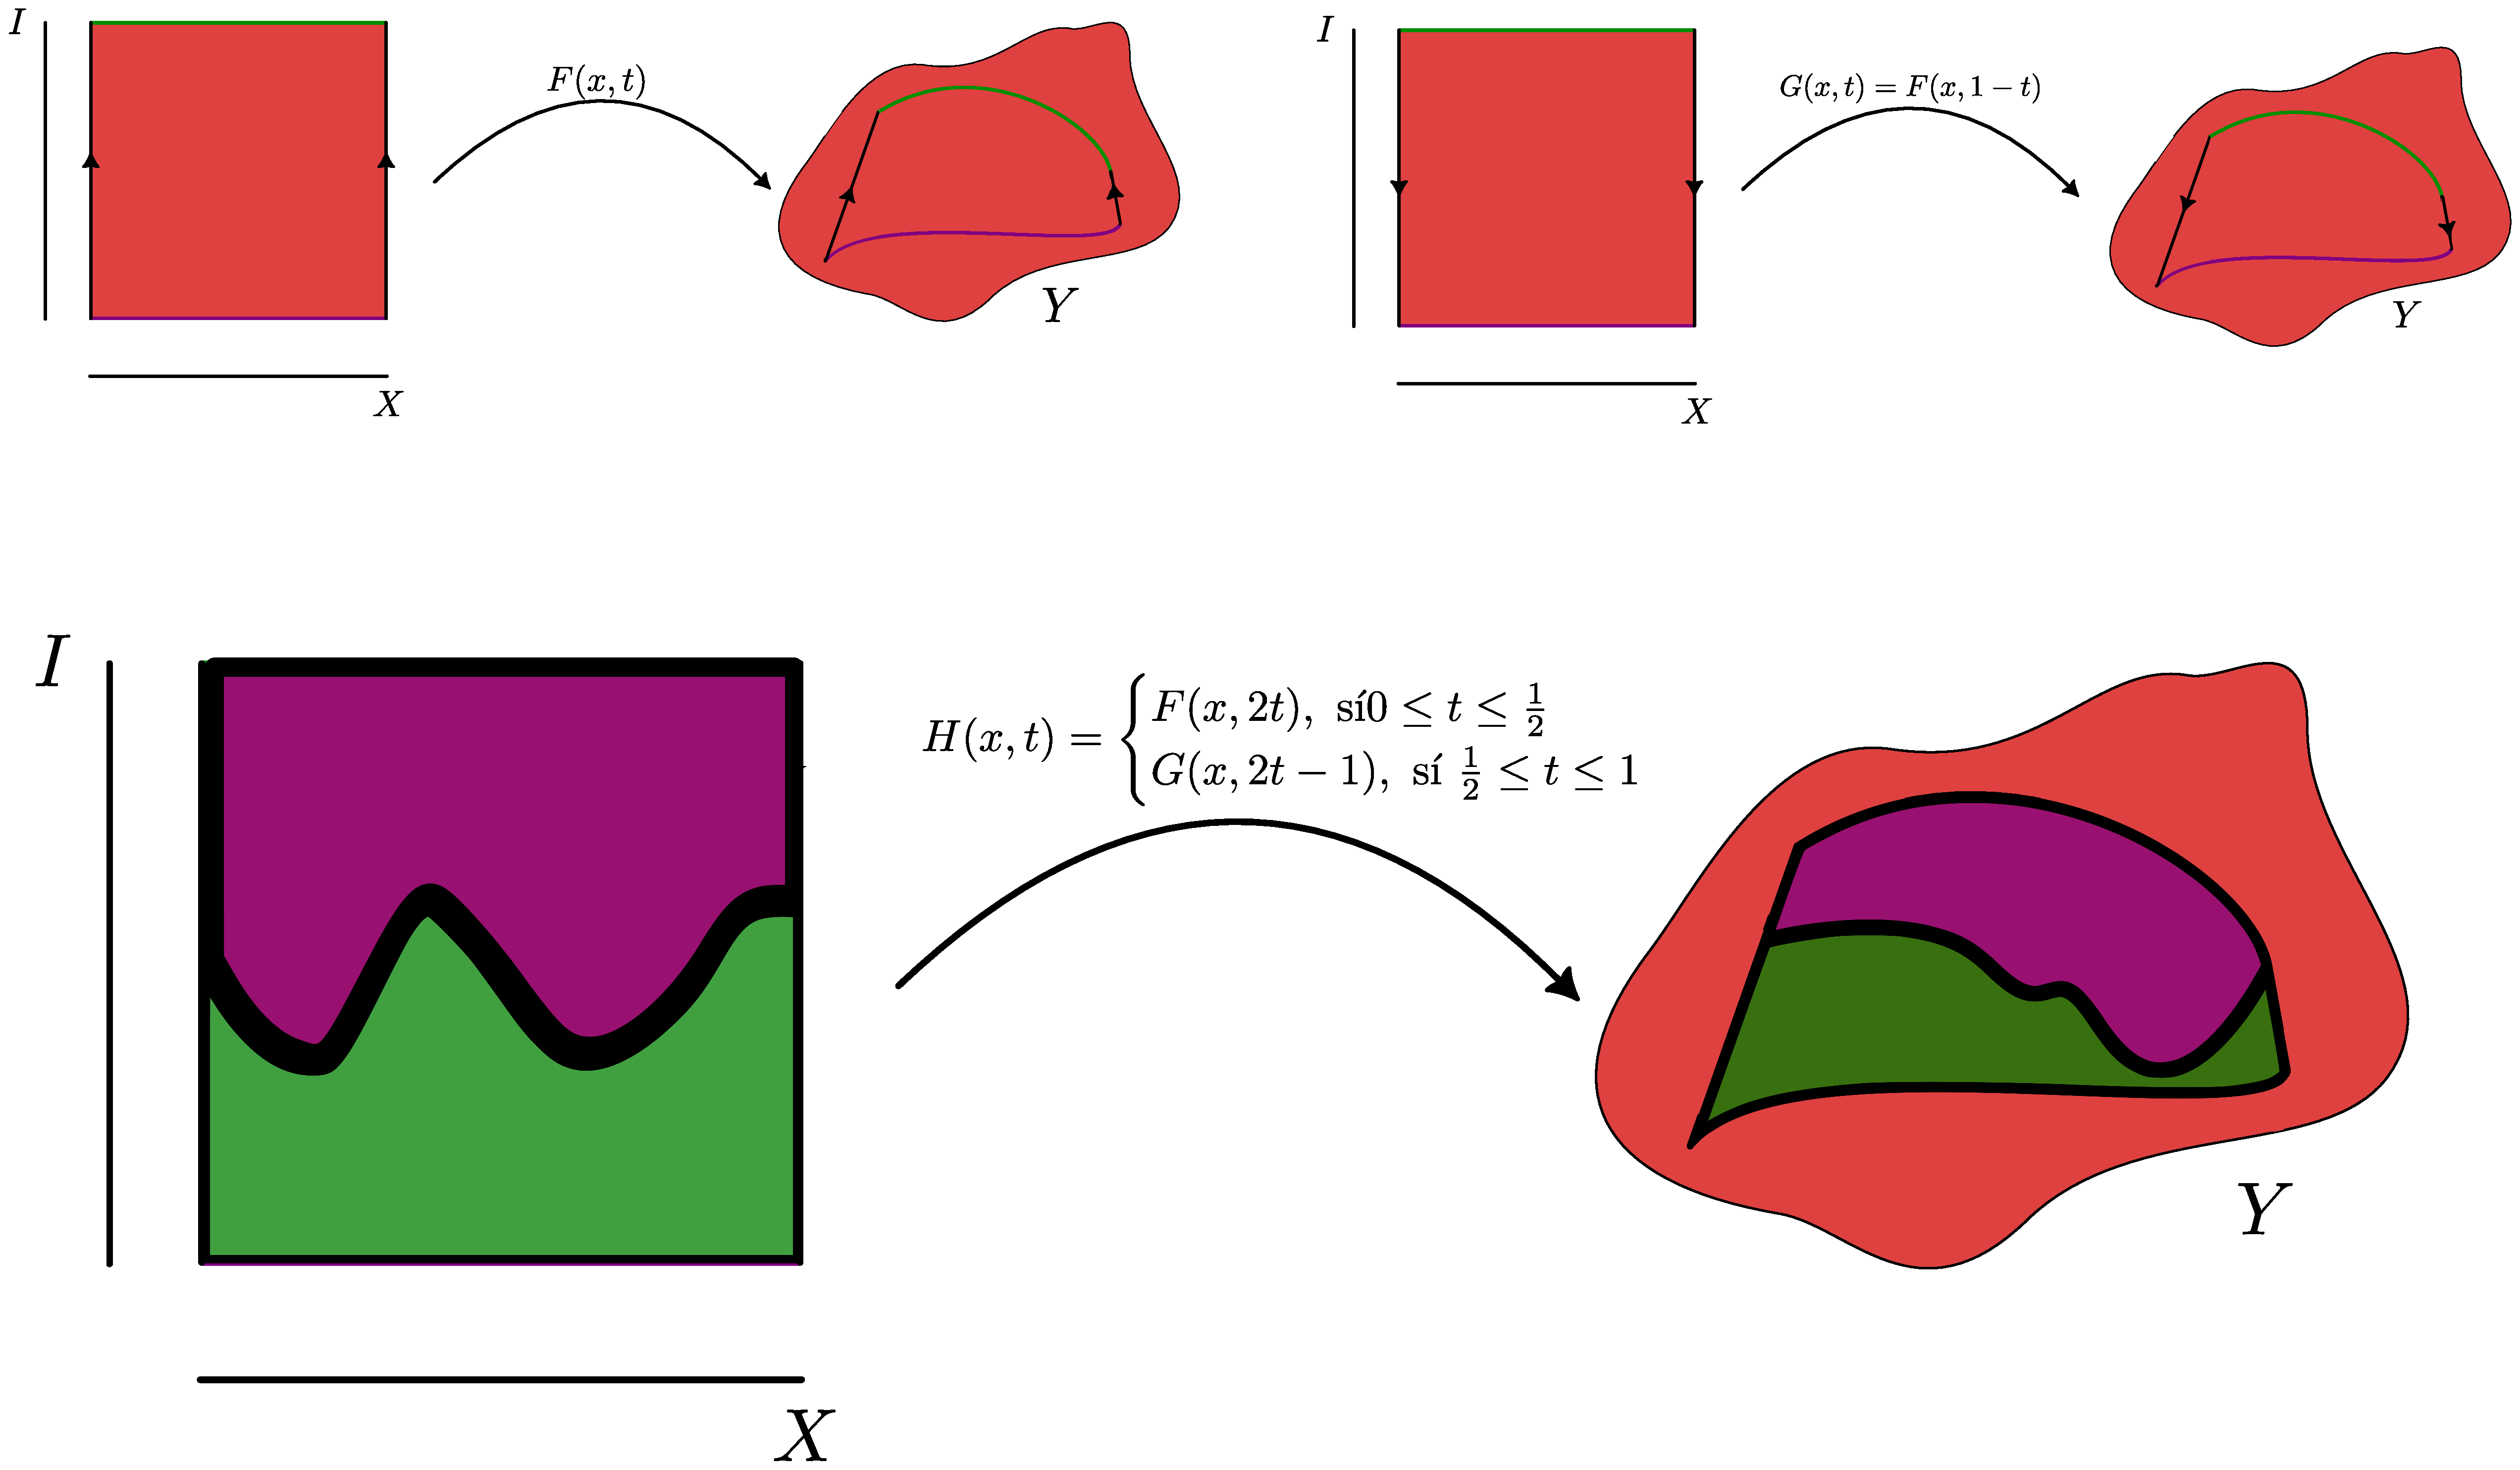
\includegraphics[scale=0.2]{Figures/homotopia_2.eps}
    \caption{La equivalencia de Homotop\'ia.}
    \label{fig_14}
\end{figure}

\begin{definition}
    Sea $X$ y  $Y$ espacios topologicos y  $f:X \xrightarrow{} Y$ una mapa
    continua. La \textbf{clase de homotop\'ia} de $f$ es el conjunto de todo
    mapa continua homotopico a $f$; es decir  $[f]=\{g:X \xrightarrow{} Y : g
    \text{ es continua y } g \simeq f\}$.
\end{definition}

\begin{theorem}\label{thm_5.10}
    Sean $X$ y  $Y$ espacios topologicos y sea  $f_i:X \xrightarrow{} Y$ y
    $g_i:X \xrightarrow{} Y$ mapas continuas para todo $i \in \faktor{\Z}{2\Z}$.
    S\'i $f_0 \simeq f_1$ y $g_0 \simeq g_1$, entonces tenemos que $g_0 \circe
    f_0 \simeq g_1 \circ f_1$.
\end{theorem}
\begin{proof}
    Sean $F:X \times I \xrightarrow{} Y$  y $G:X \times I \xrightarrow{} Y$
    homotopias entre $f_0,f_1$ y $g_0,g_1$, respectivamente. Afirmamos que $g_0
    \circ f_0 \simeq g_1 \circ f_0$. Sea $H:X \times I \xrightarrow{} Y$ la mapa
    definida como $H=G \circ f_0$. Es decir que $H(x,t)=G(f_0(x),t)$. Nota que
    como $G$ y  $f_0$ son continuas, entonces $H$ es continua, y que
    $H(x,0)=G(f_0(x),0)=g_0 \circ f_0(x)$ y $H(x,1)=G(f_0(x),1)=g_1 \circ
    f_0(x)$. As\'i que $g_0 \circ f_0 \simeq g_1 \circ f_0$.

    Ahora afirmamos que $g_1 \circ f_0 \simeq g_1 \circ f_1$. Considere $K:X
    \times I \xrightarrow{} Y$ dado por $K=g_1 \circ F$. Como $g_1$ y $F$ son
    continuas, tenemos $K$ continua. Entonces  $K(x,0)=g_1 \circ f_0(x)$ y
    $K(x,1)=g_1 \circ f_1(x)$. Entonces $g_1 \circ f_0 \simeq g_1 \circ f_1$.
    Por lo tanto, como homotopia es transitiva, obtenemos que $g_0 \circ f_0
    \simieq g_1 \circ f_1$.
\end{proof}
\begin{corollary}
    Homoto\'ia defina una congruencia en la categor\'ia $\Top$.
\end{corollary}

\begin{definition}
    Definimos el \textbf{categor\'ia homot\'opico} de ser la categor\'ia
    cociente de $\Top$ bajo homotop\'ia, y lo denotamos  $\text{hTop}$.
\end{definition}

\begin{definition}
    Una mapa continua $f:X \xrightarrow{} Y$ es una \textbf{equivalencia de
    homotop\'ia} s\'i existe un $g:Y \xrightarrow{} X$ tal que $g \circ f \simeq
    1_X$ y  $f \circ g \simeq 1_Y$. Decimos entonces que $X$ es de la misma
    \textbf{tipo de homotop\'ia} que $Y$.
\end{definition}

\begin{example}\label{}
    Un circulo y un disco perforado no son homeomorfos, per s\'i son del mismo
    tipo de homotopia.
    \begin{figure}[h]
        \centering
        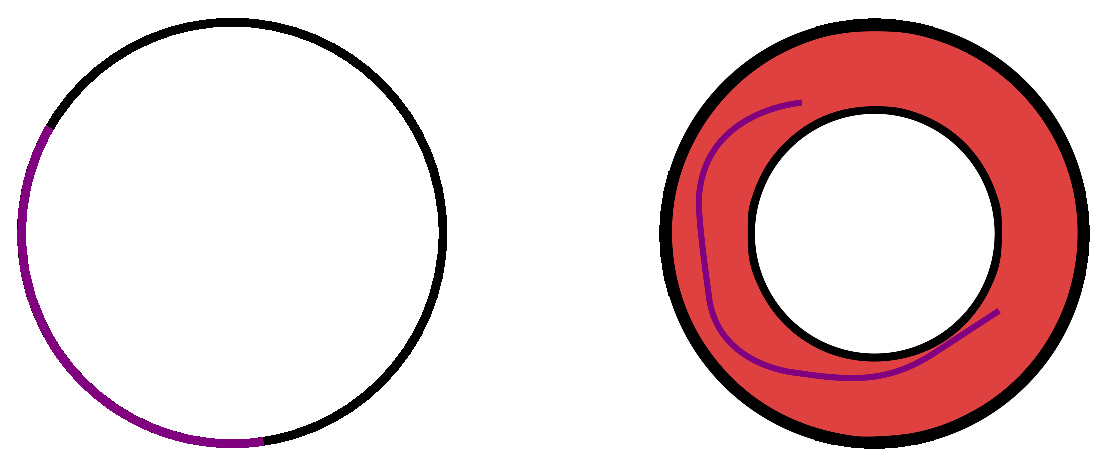
\includegraphics[scale=0.5]{Figures/homotopy_equivalence.eps}
        \caption{}
        \label{fig_15}
    \end{figure}
\end{example}

\begin{definition}
    Sean $X$ y  $Y$ espacios topologicos. Decimos que un mapa $f:X
    \xrightarrow{} Y$ es \textbf{homotopicamente nula} s\'i es homotopico a una
    mapa constante en $Y$.
\end{definition}
